\documentclass[11pt]{article}
\usepackage[utf8]{inputenc}
\usepackage[english]{babel}
\usepackage{amsmath}
\usepackage{amsfonts}
\usepackage{amssymb}
\usepackage{amsthm}
\usepackage{fullpage}
\usepackage{todonotes}
\usepackage{enumitem}
\usepackage{mathtools}
\usepackage{thmtools}
\usepackage{thm-restate}
\usepackage{booktabs}
\usepackage{url}


\newtheorem{theorem}{Theorem}[section]
\newtheorem{lemma}[theorem]{Lemma}
\newtheorem{corollary}[theorem]{Corollary}
\newtheorem{proposition}[theorem]{Proposition}
\newtheorem{claim}[theorem]{Claim}
\newtheorem{remark}[theorem]{Remark}
\newtheorem{definition}{Definition}[section]
\newtheorem{openproblem}{Open Problem}[section]


\newcommand{\lef}{\texttt{left}}
\newcommand{\righ}{\texttt{right}}
\newcommand{\gap}{\texttt{gap}}
\newcommand{\num}{\texttt{num}}
\newcommand{\out}{\texttt{out}}
\newcommand{\tup}{\texttt{tup}}

\newcommand{\mmin}{\texttt{MIN}}
\newcommand{\mmax}{\texttt{MAX}}
\newcommand{\var}{\texttt{Var}}


\begin{document}
\sloppy
\date{}
\title{Complexity of Linear Operators}
\maketitle

\begin{abstract}
Let $A \in \{0,1\}^{m \times n}$ be a~matrix with $t_0$ zeroes
and $t_1$ ones and $\mathbf{x}$ be an~$n$-dimensional vector 
over a~semigroup. How many semigroup operations are required to 
compute $A\mathbf{x}$? This problem generalizes the well-known 
range queries problem and has applications in graph algorithms, 
functional programming languages, circuit complexity, and others. It 
is immediate that $O(t_1+n+m)$ semigroup operations are 
sufficient. The main question studied in this paper is: 
can $A\mathbf{x}$ be computed using $O(t_0+n+m)$ semiring 
operations? We prove that in general this is not possible: there 
exists a~matrix $A \in \{0,1\}^{n \times n}$ having exactly two 
zeroes in every row (hence $t_0=2n$) whose complexity is 
$\Theta(n\alpha(n))$. However, for the case when the underlying 
semiring is commutative, we prove an~$O(t_0+n+m)$ upper 
bound. This implies that for commutative setting, complements 
of~sparse matrices can be processed as efficiently as spares
matrices (though the corresponding algorithm is more involved).
\end{abstract}

\thispagestyle{empty}

\section{Introduction}
\subsection{Problem Statement and New Results}
Let $A \in \{0,1\}^{m \times n}$ be a~matrix with $t_0$ zeroes
and $t_1$ ones and 
$\mathbf{x}=(x_1, \dotsc, x_n)$~be an~$n$-dimensional vector 
over a~semigroup~$(S, \circ)$. 
How many semigroup operations are required to 
compute the \emph{linear operator}~$A\mathbf{x}$?
In this case, the $i$-th element of the output vector is
$\sum_{j \colon A_{ij}=1}x_j$ where the summation 
is over the semigroup operation~$\circ$.
More generally, how many semigroup operations are needed 
to compute $AB$ where $B \in S^{n \times k}$?
In this paper, 
we are interested in lower and upper bounds 
involving~$t_0$ and~$t_1$. 
Matrices with $t_1=O(n)$ are usually called \emph{dense} 
whereas matrices with $t_2=O(n)$ 
are called \emph{complements of dense matrices}. 
It is not difficult to see that computing all $n$~outputs
of $A\mathbf{x}$ independently takes
$O(t_1+n+m)$ semigroup operations.
The main question studied in this paper is: 
can $A\mathbf{x}$ be computed using $O(t_0+n+m)$ semiring 
operations? (This complexity is easy to achieve if $\circ$ has an
easily computable inverse (in that case $S$~is a~group): in this case~$A$ can be obtained by subtracting a~dense matrix from all-ones matrix.) Our first result states that this is possible for 
\emph{commutative} semigroups.

\begin{restatable}{theorem}{upper}
\label{thm:main_statement}
Let $S$~be a~commutative semigroup, 
$\mathbf{x} \in S^{n \times 1}$ be a~vector, 
and $A \in \{0,1\}^{m \times n}$ be a~matrix with~$t_0$ zeros.
Then, $A\mathbf{x}$ can be computed using at most 
$O(m+n+t_0)$ semiring operations.
\end{restatable}

As an~immediate consequence we get the following matrix 
multiplication result.

\begin{restatable}{corollary}{matrixmult}
\label{cor:matrixmult}
Let $S$~be a~commutative semigroup, 
$A \in \{0,1\}^{n \times n}$ be a~matrix with~$t_0$ zeros,
and $B \in S^{n \times n}$ be a~matrix. Then, 
$AB$ can be computed using at most 
$O(n^2)$ semiring operations.
\end{restatable}

We then show that commutativity is essential: for 
a~strongly non-commutative semigroup~$S$ 
(the notion of strongly non-commutativity is made formal
later in the text) the minimum number of semigroup operations
needed to compute $A\mathbf{x}$ for a~matrix 
$A \in \{0,1\}^{n \times n}$ with $t_0=O(n)$ zeros is $\Theta(n\alpha(n))$ where is the inverse Ackermann function.

\begin{restatable}{theorem}{lower}
\label{thm:noncommlowerbound_statement}
For any strongly non-commutative semigroup $X$ there is a circuit to compute any dense operator of size $O(n\alpha(n))$, where $\alpha(n)$ is the inverse Ackermann function. On the other hand, there exist dense matrices~$A$ such that any circuit computing $Ax$ must have size $\Omega(n\alpha(n))$.
\end{restatable}




\subsection{Motivation}
The linear operator problem is interesting for many reasons.
\begin{description}
\item[Range queries.] In the \emph{range queries} problem, 
one is given a~vector~$\mathbf{x}=(x_1, \dotsc, x_n)$ over 
a~semiring $(S, \circ)$ and 
a~bunch of queries of the form~$(l,r)$ and is required to 
output the result $x_l \circ x_{l+1} \circ \dotsb \circ x_r$ 
for each query. The linear operator problem is thus a~natural
generalization of the range queries problem: each row of the
matrix~$A$ defines a~subset of the elements of~$\mathbf{x}$
that need to be summed up and this subset is not required to be 
a~contiguous interval. The algorithms and hardness results for 
the linear operator problem presented in this paper 
are indeed inspired 
by some of the known results for the range queries problem.
Later in the text we summarize a~rich
variety of algorithmic approaches and applications of the range 
queries problem.

\item[Graph algorithms.] Various graph path/reachability 
problems can be reduced naturally to matrix multiplication. 
Say, the all-pairs shortest path problem (APSP) is reducible
to min-plus matrix product. Another example: 
the number of triangles in an undirected graph is equal to
the trace of~$A^3$ divided by six, 
where $A$~is the adjacency matrix and matrix 
multiplication is over integers. It is natural to ask what happens if
a~graph has $O(n)$ edges or $O(n)$ anti-edges 
(as usual, by~$n$ we denote the number of nodes). 
In many cases, an efficient algorithm for sparse graphs is 
almost immediate whereas an algorithm with the same efficiency
for a~complement of a~dense graph is not so immediate. For
example, it is easy to solve APSP and triangle counting on dense graphs in time $O(n^2)$, but it is not immediate how to achieve
the same time complexity for complements of dense graphs.
In this paper, we show that the same effect occurs for linear operators: we prove that complements of dense matrices can be 
processed as efficiently as dense matrices though the corresponding algorithm is more involved. In particular, the efficient 
algorithm for matrix multiplication from Theorem~...

\item[Matrix multiplication over semirings.] Fast matrix
 multiplication methods rely essentially on the ring structure.
The first such algorithm was given by~Strassen~\cite{}, 
the current record upper bound is $O(n^{2.373})$~\cite{}; 
see the survey~\cite{} for an~overview of known approaches.
For various important semirings lacking the inverse operation, 
we still do not know an $n^{3-\varepsilon}$ upper bound for
 a~constant~$\varepsilon>0$. 
E.g., the strongest known upper bound for min-plus matrix
multiplication is $n^3/\exp(\sqrt{\log n})$. In this paper, we present natural special cases of matrices where 
faster multiplication is possible.

\item[Functional programming languages.]
%\todo{Andrey, poyasni tut, pogaluista, kak eto vsyo v functional programming ispol'zuetsya.}

\item[Circuit complexity.] Computing linear operators over
a~Boolean semiring~$(\{0,1\}, \lor)$ is a~well-studied problem 
in circuit complexity. The corresponding computational model is known as~\emph{rectifier network}. An overview of
known lower and upper bounds for such circuits is given by Jukna~\cite[Section~13.6]{DBLP:books/daglib/0028687}.
\end{description}

%\subsection{Our Contribution}
%\todo[inline]{tut budut sformulirovani nashi dve teoremi}

\subsection{Organization of the Paper}

\section{(OLD) Introduction}
Our main object of study in this paper are \emph{dense matrices}, which we
define as 0/1 matrices of size $n \times n$ that contain $O(n)$ zeroes.
%\footnote{Using this definition we slightly abuse the standard terminology as by a~dense matrix one usually means a~matrix with $\Omega(n^2)$ ones.} 
We are
interested in computations over dense matrices that take place in algebraic
structures lacking an inverse operation (e.g., semigroups and semirings).
The interest in computations over such algebraic structures has recently grew substantially throughout the
Computer Science community with the cases of Boolean and tropical semiring being of the main interest (see, for
example,~\cite{Jukna16,Williams14,butkovic10systems}).
The lack of an inverse operation sometimes changes the complexity of algorithmic problems over algebraic structure drastically and even the complexity of standard computational tasks are not well understood over tropical and Boolean semirings (see, e.g.~\cite{Williams14,GrigorievP15}). From this perspective computations over dense matrices seems to be one of the most basic questions. In the presence of an inverse operation it trivially reduces to the computations over \emph{sparse matrices}.
Without an inverse operation dense matrices
might intuitively seem harder than sparse matrices, but as we show in this paper, this intuition is
only partially correct.

Consider a \emph{dense linear operator}
\[
\mathbf{y} = A\mathbf{x},
\]
where $A$ is a dense matrix and~$\mathbf{x}=(x_1, \cdots, x_n)$ is a vector over
an arbitrary semigroup (see Section~\ref{subsec:algstr} for definitions
and examples of algebraic structures used in this paper). $(S, \circ)$. Our goal
is to simultaneously compute all elements of the resulting vector
$\mathbf{y}=(y_1, \cdots, y_n)$, where

\begin{equation}\label{eq-sum}
y_i = \sum_{A_{ij}=1} x_j
\end{equation}

\noindent
for all $1 \le i \le n$, and the ``summation'' is over the semigroup operation
$\circ$. What is the size of the smallest circuit comprising 2-input gates
$\circ$ that computes $\mathbf{y}$?

Note that if $A$ is sparse, i.e. contains $O(n)$ ones, then~(\ref{eq-sum})
directly yields a linear-size circuit. Furthermore, if the summation is over a
\emph{commutative group} rather than just a semigroup, then the dense case can
be reduced to the sparse one by \emph{subtracting} $y_i$ from the sum
$x_1 \circ \cdots \circ x_n$. A similar reduction is also not hard to show for the case of non-commutative groups.

A natural solution that first comes to mind in the semigroup case is to split
the rows of the matrix $A$ into ranges of consecutive ones, thus obtaining
$O(n)$ ranges overall, and then apply the classic \emph{Range Queries} algorithm
by Yao~\cite{DBLP:conf/stoc/Yao82} to compute all ranges by a circuit of size
$O(n\alpha(n))$, where $\alpha(n)$ is the inverse Ackermann function, and
subsequently combine the results with $O(n)$ additional gates.

Can we do better? In general, the answer is ``No''. However, if the semigroup is
\emph{commutative}, the answer is, remarkably, ``Yes''! We present a linear-size
circuit construction for dense linear operators in Section~\ref{sec-commutative}.
Furthermore, in Section~\ref{sec-non-commutative}
we prove that the
% Volodya, I removed "(both commutative and non-commutative versions of)" from
% here, because I think it's a premature but distracting detail at this stage.
non-commutative case is equivalent to the Range Queries problem that, as shown
by Chazelle and Rosenberg~\cite{DBLP:journals/ijcga/ChazelleR91}, requires
$\Theta(n\alpha(n))$ gates, hence separating the complexity of the two cases.

% A counterintuitive corollary of our separation theorem is that the case of
% non-commutative groups is strictly harder than the case of commutative
% semigroups. In other words, inverses provide no additional power for the studied
% problem, whereas commutativity does.

%As an additional contribution, we prove that the same bound
% $\Theta(n\alpha(n))$ also holds for the case of \emph{idempotent}
% non-commutative semigroups, which are significantly more powerful.




\paragraph{Organization of the paper.} Section~\ref{sec-background} provides basic definitions used throughout the
paper. Section~\ref{sec-applications} highlights applications of the
presented linear-size construction. In particular, we observe that an
$n\times n$ matrix can be multiplied by a dense matrix over an arbitrary
semiring in $O(n^2)$ time. This appears to be significantly more challenging
compared to the case of multiplication over a \emph{ring}, which can reduced to
sparse matrix multiplication via subtraction. In Section~\ref{sec:statement} we give the precise statements of our results.

\section{Background}\label{sec-background}

In this section we review basic algebraic structures used in this paper, as well
as the classic Range Queries problem that turns out to be inherently related to
dense linear operators.

\input algebraic_structures

\subsection{Range Queries problem}
{\em Range Queries} is a~classical problem in data structures and algorithms
having a~variety of applications in fields like bioinformatics and string
algorithms, computational geometry, image analysis, real-time systems, and
others (we review some of the applications in Subsection~\ref{subseq:rmqapp}, as
well as a~rich variety of algebraic techniques for the problem in
Subsection~\ref{subsec:approaches}).

In the Range Queries problem, one is given a~sequence $x_1, x_2, \dotsc, x_n$ of
elements of a fixed semigroup $(S, \circ)$. Then, a~\emph{range query} is
specified by a pair of indices $(l,r)$, such that $1 \le l \le r \le n$. The
answer to such a~query is the result of applying the semigroup operation to the
corresponding range, i.e., $x_l \circ x_{l+1} \circ \dotsb \circ x_r$. The Range
Queries problem is then to simply answer all given range queries. There are two
regimes: online and offline. In the {\em online regime}, one is given
a~sequence of {\em values} $x_1=v_1, x_2=v_2, \dotsc, x_n=v_n$ and is asked to preprocess it so that to
answer efficiently any subsequent query. By ``efficiently'' one usually
means in time independent of the length of the range (i.e., $r-l+1$, the time
of a~naive algorithm), say, in time $O(\log n)$ or $O(1)$. In this paper, we
focus on the {\em offline} version, where one is given a~sequence together with
all the queries, and are interested in the minimum number of semigroup
operations needed to answer all the queries. Moreover, we study a~more general
problem: we assume that $x_1, \dotsc, x_n$ are formal variables rather than
actual semigroup values. That is, we study the circuit size of the corresponding
computational problem (the formal definition of the computational model is given
later in the text).

% TODO: In the final version, show that the Range Queries problem becomes
% trivial for a commutative group. Also, what about non-commutative groups?

\section{Motivation and Applications}\label{sec-applications}

In this section we discuss our motivation and demonstrate two applications of
the presented linear-size construction for a dense linear operator: fast
multiplication of dense and \emph{boring} matrices over arbitrary semirings
(Section~\ref{sec-boring-matrices}) and compact algebraic representation of
dense graphs (Section~\ref{sec-dense-graph}).

\subsection{Dense Operators}

Throughout this section we consider $n \times n$ matrices over an arbitrary
semiring $(S, \circ, \bullet)$, where the operations $\circ$ and $\bullet$ have
identities 0 and 1, respectively.

A matrix is \emph{sparse} if most of its elements are 0. To be more precise, we
further assume that a sparse matrix has $O(n)$ non-zero elements. Sparse
matrices arise in many applications, and can be multiplied by arbitrary vectors
in $O(n)$ time and arbitrary matrices in $O(n^2)$ time (multiplication
by an $n\times n$ matrix can be thought of as multiplication by $n$ vectors).
% Note that these complexity bounds are exact, as they match the time required to
% read the input.

A \emph{0/1 matrix} is a matrix whose elements belong to the set $\{0,1\}$. A
0/1 matrix is \emph{dense} if it has $O(n)$ zero elements, i.e. most of its
elements are 1.

Note that multiplication of dense matrices by vectors can be viewed as a special
case of the Range Queries problem. Indeed, we can split the rows of a dense
matrix into $O(n)$ ranges, compute answers to these range queries, and then
recover the rows by combining the constituent ranges.

As mentioned above, computations on dense matrices over algebraic structures
with inverse operations can often be reduced to computations on sparse matrices.
However, the situation changes for computations over semigroups or semirings,
which lack inverse operations. In such cases, the computation complexity of
various matrix operations can differ significantly from more classical settings,
which is a recurring topic in the recent years (see, for
example,~\cite{AkianGG12,Williams14,GrigorievP15}). This paper provides further
insight on this topic. As far as we know, the complexity of the problem under
consideration was not known even for the simplest semigroups like
$(\mathbb{B},\vee)$.

\subsection{Dense and boring matrix multiplication}\label{sec-boring-matrices}

Out first main result presented in Section~\ref{sec-commutative} allows us to
obtain a linear-size circuit for multiplying a 0/1~dense matrix of size
$n \times n$ by a vector in an arbitrary semiring. Our construction is explicit
and the corresponding algorithm takes $O(n^2)$ time (faster
implementations are possible if the input matrix is provided in a compressed
form). As a consequence, we can multiply a 0/1~dense matrix $A$ by an arbitrary
matrix $B$ in $O(n^2)$ time as follows:

\begin{itemize}
  \item Construct a linear-size circuit for the dense linear operator
  $A\mathbf{x}$. Time complexity: $O(n^2)$.
  \item Evaluate the circuit on all $n$ columns of the matrix $B$. Each
  evaluation takes $O(n)$ time, hence the overall time complexity of this step
  is also $O(n^2)$.
\end{itemize}

Furthermore, by combining the algorithms for sparse and dense matrix
multiplication, one can obtain an efficient algorithm for the multiplication of
so-called \emph{boring} matrices.

A matrix is \emph{boring} if most of its elements are equal to some element~$b$ from
the semiring. To be more precise, we further assume that a boring matrix has
$O(n)$ elements that are not equal to~$b$. Boring matrices are a natural
generalisation of sparse and dense matrices: both are just special cases with
$b=0$ and $b=1$, respectively.

To multiply a boring matrix $A$ by a vector $\mathbf{x}$, we decompose the
matrix into two components $A_0$ and $A_1$, such that $A = A_0 \circ b A_1$,
$A_0$ is sparse, and $A_1$ is dense (note that here the operations
$\circ$ and $\bullet$ (the latter is represented by juxtaposition) are lifted to
matrices). Now we can compute $A \mathbf{x}$ thanks to various semiring laws:

\[
\begin{array}{rcll}
A \mathbf{x} & = & (A_0 \circ b A_1) \mathbf{x} & \text{(sparse-dense decomposition)}\\
 & = & A_0 \mathbf{x} \circ (b A_1) \mathbf{x} & \text{(distributivity and commutativity)}\\
 & = & A_0 \mathbf{x} \circ b (A_1 \mathbf{x}) & \text{(associativity)}\\
\end{array}
\]

\noindent
Both $A_0 \mathbf{x}$ and $A_1 \mathbf{x}$ can be computed using sparse and
dense matrix-vector multiplication, respectively; the results are further
combined using scalar multiplication by $b$ and vector addition $\circ$, both of
which take linear time and have linear-size circuits. Note that the second step
in the above equation relies on commutativity in a crucial way: elements of the
original matrix $A$ are partitioned into elements of $A_0$ and $A_1$ in an
arbitrary order. As in the dense case, this immediately leads to $O(n^2)$-time
boring matrix multiplication.

\subsection{Dense graph representation}\label{sec-dense-graph}

Let us revisit the graph semigroup defined in Section~\ref{subsec:algstr}.
We will denote it by $(G_U, +)$, where $G_U$ is the set of directed graphs whose
vertices come from a universe $U$, that is, if $(V, E) \in G_U$ then
$V \subseteq U$ and $E \subseteq V \times V$. Recall that the graph overlay
operation $+$ is defined as

\[
(V_1, E_1) + (V_2, E_2) = (V_1 \cup V_2, E_1 \cup E_2).
\]

\noindent
The algebra of graphs presented in~\cite{mokhov2017algebraic} also defines
the \emph{graph connect} operation $\rightarrow$:
% \footnote{The definition
% coincides with that of \emph{graph join}~\cite{1969_graph_theory_harary}, but,
% just like graph union, graph join requires that given graphs are
% non-overlapping. The connect operation has no such requirement.}

\[
(V_1, E_1) \rightarrow (V_2, E_2) = (V_1 \cup V_2, E_1 \cup E_2 \cup V_1 \times V_2).
\]

This operation allows us to ``connect'' two graphs by adding edges from every
vertex in the left-hand graph to every vertex in the right-hand graph, possibly
introducing self-loops if $V_1 \cap V_2 \neq \emptyset$. The operation is
associative, non-commutative and distributes over $+$. Note, however, that the
empty graph $\varepsilon = (\emptyset, \emptyset)$ is the identity for both
overlay and connect operations: $\varepsilon + x = x + \varepsilon = x$ and
$\varepsilon \rightarrow x = x \rightarrow \varepsilon = x$, and consequently
the annihilating zero property does not hold, which makes this algebraic
structure not a~semiring according to the classic semiring definition.

By using the two operations one can construct any graph starting from primitive
single-vertex graphs. For example, let $U=\{1,2,3\}$ and $k$ stand for a
single-vertex graph $({k}, \emptyset)$. Then:

\begin{itemize}
  \item $1 \rightarrow 2$ is the graph comprising a single edge $(1,2)$, i.e.
  $1 \rightarrow 2 = (\{1,2\}, \{(1,2)\})$.
  \item $1 \rightarrow (2 + 3)$ is the graph $(\{1,2,3\}, \{(1,2),(1,3)\})$.
  \item $1 \rightarrow 2 \rightarrow 3$ is the graph $(\{1,2,3\}, \{(1,2),(1,3),(2,3)\})$.
\end{itemize}

\noindent
Clearly any sparse graph $(V, E)$, i.e. a graph with a sparse connectivity
matrix, can be constructed by a linear-size expression:

\[
(V, E) = \sum_{v \in V} v + \sum_{(u,v) \in E} u \rightarrow v.
\]

\noindent
But what about complements of sparse graphs, i.e. graphs with dense
connectivity matrices? It is not difficult to show that by applying the dense
linear operator we can obtain a linear-size circuit comprising 2-input gates
$+$ and $\rightarrow$ for any dense graph.

Let $A$ be a dense matrix of size $n\times n$. Our goal is to construct the
graph $G_A = (\{1, \dots, n\}, E)$ such that $(i,j) \in E$ whenever $A_{ij}=1$.

First, we compute the dense linear operator $\mathbf{y} = A \mathbf{x}$ over the
(commutative) graph semigroup~$+$, where $\mathbf{x} = (1, 2, \dots, n)$, i.e.,
$x_j$ is the primitive graph comprising a single vertex~$j$, obtaining
graphs~$y_i$ that comprise sets of isolated vertices corresponding to the rows
of matrix~$A$:

\[
y_i = \sum_{A_{ij}=1} j \, .
\]

The resulting graph $G_A = (\{1, \dots, n\}, E)$ can now be obtained by using
the connect operation~$\rightarrow$ to connect $i$ to all vertices $y_i$, and
subsequently overlaying the results:

\[
G_A = \sum_{i=1}^{n} i \rightarrow y_i.
\]

Thanks to the linear-size construction for the dense linear operator, the size
of the circuit computing $G_A$ is $O(n)$. This allows us to store dense graphs
on $n$ vertices using $O(n)$ memory, and perform basic transformations of dense
graphs in $O(n)$ time. We refer the reader to~\cite{mokhov2017algebraic} for
further details about applications of algebraic graphs in functional programming
languages.

\section{Computational Model}

In this section we define our computational model, which includes a few less
commonly known notions related to semigroups, as well as semigroup circuits.

\subsection{Faithful semigroups}
%\todo[inline]{Volodya, mogesch', pogalauista, etu podsektsiyu perenesti v sektsiyu 6? Ved' eto vsyo nugno rovno dlya dok-va nignei otsenki v sektsii 6.}

In the paper we consider computations over general semigroups. To establish
complexity results and especially to establish reasonable lower bounds we need
to consider semigroups with relatively rich structure.

Since we deal with computations with formal semigroup variables, it is
convenient to introduce the following notation. Suppose $(S, \circ)$ is a
semigroup. Let $X_{S,n}$ be a semigroup with generators $\{x_1,\ldots, x_n\}$
and with the equivalence relation consisting of identities in variables
$\{x_1,\ldots, x_n\}$ over~$(S,\circ)$. That is, for two words $W$ and $W'$ in
the alphabet $\{x_1,\ldots,x_n\}$ we have $W=W'$ in $X_{S,n}$ iff no matter which
elements of the semigroup~$S$ we substitute for $\{x_1,\ldots, x_n\}$ we obtain
a~correct equation over~$S$. In particular, note that if $S$~is commutative
(respectively, idempotent), then $X_{S,n}$ is also commutative (respectively,
idempotent). We will often omit the subscript $n$ and write simply $X_S$ since the number of generators will be clear from the context.

Below we will use the following notation. Let $W$ be a word in the alphabet
$\{x_1,\ldots, x_n\}$. Denote by $\var(W)$ the set of letters that are present
in $W$.

The case of general commutative semigroups and computations over them was
previously studied in relation to the Range Queries problem. The standard
approach to capture their generality here is to consider \emph{faithful
commutative semigroups}~\cite{DBLP:conf/stoc/Yao82,DBLP:journals/ijcga/ChazelleR91}.

\begin{definition}
A commutative semigroup $(S, \circ)$ is \emph{faithful commutative} if for any
equivalence $W\sim W'$ in $X_S$ we have $\var(W)=\var(W')$.
\end{definition}

Note that this definition does not pose any restrictions on the cardinality of
each letter in $W$ and $W'$. This allows us to capture in this definition
important cases of idempotent semigroups. For example, semigroups
$(\{0,1\}, \vee)$ and $(\mathbb{Z},\min)$ are commutative faithful.

We also need to study the non-commutative case, and moreover, our results
establish the difference between commutative and non-commutative cases. Thus,
we need to extend the notion of faithfulness to non-commutative semigroups to
capture their non-commutativity in the whole power. At the same time we would
like to keep the case of idempotency. We introduce the notion of faithfulness
for the non-commutative case inspired by the properties of free idempotent
semigroups~\cite{GreenR52}. To introduce this notion we need several
definitions.

The \emph{initial mark} of $W$ is the letter that is present in $W$ such that
its first appearance is farthest to the right. Let $U$ be the prefix of $W$
consisting of letters preceding the initial mark. That is, $U$ is the maximal
prefix of $W$ with a smaller number of generators. We call $U$ the
\emph{initial} of $W$. Analogously we define the \emph{terminal mark} of $W$ and
the \emph{terminal} of $W$.

\begin{definition}\label{def:strong_non_commutativity}
We say that a semigroup $X$ with generators $\{x_1,\ldots, x_n\}$ is
\emph{strongly non-commutative} if for any words $W$ and $W'$ in the
alphabet $\{x_1,\ldots, x_n\}$ the equivalence $W\sim W'$ holds in $X$ only if
the initial marks of $W$ and $W'$ are the same, terminal marks are the same,
the equivalence $U \sim U'$ holds in $X$, where $U$ and $U'$ are the initials of
$W$ and $W'$, respectively, and the equivalence $V \sim V'$ holds in $X$, where
$V$ and $V'$ are the terminals of $W$ and $W'$, respectively.
\end{definition}

In other words, this definition states that the first and the last occurrences
of generators in the equivalence separates the parts of the equivalence that
cannot be affected by the rest of the generators and must therefore be the
equivalences themselves. We also note that this definition exactly captures the
idempotent case: for a free idempotent semigroup the condition in this
definition is ``if and only if''\cite{GreenR52}.

\begin{definition} \label{def:faithful}
A semigroup $(S, \circ)$ is \emph{faithful} if $X_S$ is strongly non-commutative.
\end{definition}

We note that this notion of faithfulness is relatively general and is true for
semigroups $(S,\circ)$ with considerable degree of non-commutativity in their
structure. It clearly captures free semigroups with at least two generators. It is also easy to see that the
requirements in Definition~\ref{def:faithful} are satisfied for the free
idempotent semigroup with $n$ generators (if $S$ is idempotent, then $X_S$ is also
clearly idempotent and no other relations are holding in $X_S$ since we can
substitute generators of $S$ for $x_1, \ldots, x_n$).

Next we observe some properties of strongly non-commutative semigroups that we
need in our constructions.

\begin{lemma} \label{lem:prefix_equivalence}
Suppose $X$ is strongly non-commutative. Suppose the equivalence $W \sim W'$
holds in~$X$ and $|\var(W)|=|\var(W')|=k$. Suppose $U$~and~$U'$ are minimal
(maximal) prefixes of $W$ and $W'$ such that $|\var(U)| = |\var(U')| = l\leq k$.
Then the equivalence $U \sim U'$ holds in $X$. The same is true for suffixes.
\end{lemma}

\begin{proof}
The proof is by induction on the decreasing $l$. Consider the maximal prefixes
first. For $l=k$ and maximal prefixes we just have $U=W$ and $U'=W'$. Suppose
the statement is true for some $l$, and denote the corresponding prefixes by $U$
and $U'$, respectively. Then note that the maximal prefixes with $l-1$ variables
are initials of $U$ and $U'$. And the statement follows by
Definition~\ref{def:strong_non_commutativity}.

The proof of the statement for minimal prefixes is completely analogous. Note
that on the step of induction the prefixes differ from the previous case by one
letter that are initial marks of the corresponding prefixes. So these additional
letters are also equal by the Definition~\ref{def:strong_non_commutativity}.

The case of suffixes is completely analogous.
\end{proof}

The next lemma is a simple corollary of Lemma~\ref{lem:prefix_equivalence}.
\begin{lemma} \label{lem:variables_order}
Suppose $X$ is strongly non-commutative. Suppose $W \sim W'$ holds in $X_S$. Let us write down the letters of $W$ in the order in which they appear first time in $W$ when we read it from left to right. Let's do the same for $W'$. Then we obtain exactly the same sequences of letters.

The same is true if we read the words from right to left.
\end{lemma}

\subsection{Circuits}
We assume that the input consists of $n$~formal variables
$\{x_1, \dotsc, x_n\}$. We are interested in the minimum number of semigroup
operations needed to compute all given words $\{w_1, \dotsc, w_m\}$ (e.g., for
the range queries problem, each word has a~form $x_l\circ x_{l+1}\circ \dotsb \circ x_r$). We use
the following natural {\em circuit} model. A~circuit computing all these queries
is a~directed acyclic graph. There are exactly $n$~nodes of zero in-degree. They
are labelled with $\{x_1, \dotsc, x_n\}$ and are called {\em input gates}. All
other nodes have positive in-degree and are called {\em gates}. Finally, some
$m$~gates have out-degree~0 and are labelled as {\em output gates}. The
{\em size} of a~circuit is its number of edges (also called {\em wires}). Each
gate of a~circuit computes a~word defined in a~natural way: input gates compute
just $\{x_1, \dotsc, x_n\}$; any other gate of in-degree~$r$ computes a~word
$f_1 \circ f_2 \circ \dotsb \circ f_r$ where $\{f_1, \dotsc, f_r\}$ are words
computed at its predecessors (therefore, we assume that there is an underlying
order on the incoming wires for each gate). We say that the circuit computes the
words $\{w_1, \dotsc, w_m\}$ if the words computed at the output gates are
equivalent to $\{w_1, \dotsc, w_m\}$.

For example, the following circuit computes range queries $(l_1,r_1)=(1,4)$ and
$(l_2,r_2)=(2,5)$ over inputs $\{x_1, \dotsc, x_5\}$ or, equivalently, the
linear operator $A\mathbf{x}$ where
$A=\begin{pmatrix}1&1&1&1&0\\0&1&1&1&1\end{pmatrix}$ and
$\mathbf{x}=(x_1, \dotsc, x_5)^T$.

\begin{center}
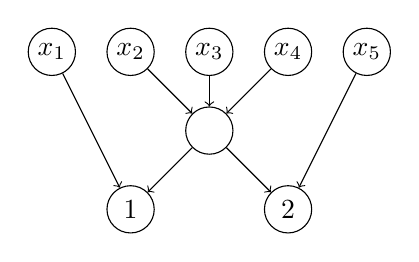
\begin{tikzpicture}
%\draw[help lines] (0,0) grid (10,6);
\foreach \x/\y/\n/\t in {0/4/x1/x_1, 1/4/x2/x_2, 2/4/x3/x_3, 3/4/x4/x_4, 4/4/x5/x_5, 2/3/a/~, 1/2/b/1, 3/2/c/2}
  \node[inner sep=0mm,circle,draw,minimum size=6mm] (\n) at (\x,\y) {$\t$};
\foreach \s/\t in {x2/a, x3/a, x4/a, a/b, x1/b, a/c, x5/c}
  \draw[->] (\s) -- (\t);
\end{tikzpicture}
\end{center}

For a~0/1-matrix~$A$, by $C(A)$ we denote the \emph{minimum number of gates} in
a~circuit computing the linear operator $A\mathbf{x}$.


A~{\em binary circuit} is a~circuit having no gates of fan-in more than two. It
is not difficult to see that any circuit can be converted into a~binary circuit
of size at most twice the size of the original circuit. For this, one just
replaces every gate of fan-in~$k$, for $k>2$, by a~binary tree with $2k-2$ wires
(such a~tree contains $k$~leaves hence $k-1$ inner nodes and $2k-2$ edges).

Clearly, in the binary circuit the number of gates does not exceed its size
(i.e., the number of wires). And the number of gates in a~binary circuit is
exactly the minimum number of semigroup operations needed to compute the
corresponding function.

Note that we can view circuits as computations over some semigroup $(S,\circ)$,
meaning that we can substitute instead of the variables elements of the
semigroup $S$. If we fix some semigroup $(S,\circ)$ we can actually consider a
circuit as a computation in the semigroups $X_S$. Moreover, we can forget about
the original semigroup $S$ and consider the computations in the circuit as
computations in an arbitrary semigroup $X$ with generators
$\{x_1, \ldots, x_n\}$.

In an~important special case of the Boolean semigroup $(\{0,1\}, \lor)$,
circuits we are discussing are known as {\em rectifier networks}. An overview of
known lower and upper bounds for such circuits is given by Jukna
in~\cite[Section~13.6]{DBLP:books/daglib/0028687}.



\end{document}